\def\urlSite{https://brevet.initiation.aero}

\ifdefined\activerhandout 
\documentclass[12pt,aspectratio=1610,handout]{beamer}
\else
\documentclass[12pt,aspectratio=1610]{beamer}
\fi

\usepackage[
    backend=biber,
    %style=authoryear-icomp,
    style=numeric,
    %style=ieee,
    sortlocale=fr_FR,
    natbib=true,
    url=true, 
    doi=true,
    eprint=true
]{biblatex}
	\addbibresource{commun/biblio.bib}
	\addbibresource{01-EtudeAeronefs/biblio.bib}
	\addbibresource{02-Navigation/biblio.bib}
	\addbibresource{03-Meteo/biblio.bib}
	\addbibresource{04-Aerodynamique/biblio.bib}
	\addbibresource{05-Histoire/biblio.bib}
	\addbibresource{Annexes/biblio.bib}
	\addbibresource{Annexes/friseChronologique/biblio.bib}
	\addbibresource{Annexes/friseChronologique/extraitsVideo/biblio.bib}

%\usepackage[french]{babel} %=> erreur avec les tikz du moteur
\usepackage[T1]{fontenc}
\usepackage[utf8]{inputenc}
\usepackage{lmodern}
\usepackage{hyperref}
\usepackage{smartdiagram}
\usepackage{xcolor}
\usepackage{tikz}
\usepackage{animate}
\usepackage{tikzpeople}
\usepackage{appendixnumberbeamer}
\usepackage[labelformat=empty]{caption}
%\usepackage{pictochrono}
\usepackage{fontawesome5}
\usepackage{awesomebox}
\usepackage{siunitx}
\usepackage{icomma}
\usepackage{physics}
\usepackage[pdftex,outline]{contour} % glow around text
\usepackage{ifthen}
\usepackage{fp}
\usepackage{textcomp}
\usepackage{gensymb}

\usetheme{Warsaw}
\setbeamertemplate{page number in head/foot}[totalframenumber]

\newcommand{\anglais}[1]{(\textit{\color{blue}#1})}
\newcommand{\legende}[2]{\caption{#1\ifdefined\activerbibliobeamer \cite{#2}\fi}}
\newcommand{\histoire}[1]{\begin{awesomeblock}{2pt}{\faBook}{black!75}#1\end{awesomeblock}}
\newcommand{\info}[1]{\begin{awesomeblock}{2pt}{\faInfoCircle}{blue!75}#1\end{awesomeblock}}
\newcommand{\question}[1]{\begin{awesomeblock}{2pt}{\faQuestionCircle}{black!75}#1\end{awesomeblock}}
\newcommand{\alerte}[1]{\begin{awesomeblock}{2pt}{\faExclamationCircle}{red!75}#1\end{awesomeblock}}
\newcommand{\astuce}[1]{\begin{awesomeblock}{2pt}{\faLightbulb}{black!75}#1\end{awesomeblock}}
\newcommand{\exemple}[1]{\begin{awesomeblock}{2pt}{\faSearch}{black!75}#1\end{awesomeblock}}
\newcommand{\definitionAConnaitre}[1]{\begin{awesomeblock}{2pt}{\faCog}{black!75}#1\end{awesomeblock}}

%\newcommand{\qmcBia}[8]{
%%1 : titre slide
%%2 : numéro de la bonne réponse
%%3 : Inititulé de la question
%%4, 5, 6, et 7 : propositions de réponse
%%8 : explication
%\begin{frame}{#1}
%\begin{awesomeblock}{2pt}{\faQuestion}{black!75}
%#3
%	\begin{enumerate}
%	\ifnum#2=1
%		\only<1>{\item #4}
%		\only<2>{\item \textbf{#4}}
%	\else
%		\item #4
%	\fi
%	\ifnum#2=2
%		\only<1>{\item #5}
%		\only<2>{\item \textbf{#5}}
%	\else
%		\item #5
%	\fi
%	\ifnum#2=3
%		\only<1>{\item #6}
%		\only<2>{\item \textbf{#6}}
%	\else
%		\item #6
%	\fi
%	\ifnum#2=4
%		\only<1>{\item #7}
%		\only<2>{\item \textbf{#7}}
%	\else
%		\item #7
%	\fi
%	\end{enumerate}
%	\pause
%\end{awesomeblock}
%#8
%\end{frame}
%}

\newcommand{\qmcBia}[8]{
%1 : titre slide
%2 : numéro de la bonne réponse
%3 : Inititulé de la question
%4, 5, 6, et 7 : propositions de réponse
%8 : explication
\begin{frame}{#1}
\begin{awesomeblock}{2pt}{\faQuestion}{black!75}
#3
	\begin{enumerate}
	\item #4
	\item #5
	\item #6
	\item #7
	\end{enumerate}
\end{awesomeblock}
\end{frame}

\begin{frame}{#1}
\begin{awesomeblock}{2pt}{\faQuestion}{black!75}
#3
	\begin{enumerate}
	\ifnum#2=1
		\item \textbf{#4}
	\else
		\item #4
	\fi
	\ifnum#2=2
		\item \textbf{#5}
	\else
		\item #5
	\fi
	\ifnum#2=3
		\item \textbf{#6}
	\else
		\item #6
	\fi
	\ifnum#2=4
		\item \textbf{#7}
	\else
		\item #7
	\fi
	\end{enumerate}
\end{awesomeblock}
#8
\end{frame}
}

\subtitle{BIA - Brevet d'Initiation Aéronautique}
%\author[BIA]{Clément \textsc{Vermot-Desroches}}
\author[BIA]{\urlSite}
\institute{Collège Aliénor d'Aquitaine\\Martignas-sur-Jalle}
%\date{\today}
\date{Année 2026-2027}

\AtBeginSection[]
{
    \begin{frame}
        %\frametitle{Table of Contents}
        \tableofcontents[currentsection]
    \end{frame}
}

\AtBeginSubsection[]
{
    \begin{frame}
        %\frametitle{Table of Contents}
        \tableofcontents[currentsection,currentsubsection]
    \end{frame}
}

%%%%%%%%%%%%%%%%%%%%%%%%%%%%%%%%%%%%%%%%%%%%%%%%%%%%%%%%%%%%%%%%%%%%%%%%%%%%%%
% \embedvideo{<poster or text>}{<video file (MP4+H264)>}
% \embedvideo*{...}{...}                     % auto-play
%%%%%%%%%%%%%%%%%%%%%%%%%%%%%%%%%%%%%%%%%%%%%%%%%%%%%%%%%%%%%%%%%%%%%%%%%%%%%%
\usepackage[bigfiles]{pdfbase}
\ExplSyntaxOn
\NewDocumentCommand\embedvideo{smm}{
  \group_begin:
  \leavevmode
  \tl_if_exist:cTF{file_\file_mdfive_hash:n{#3}}{
    \tl_set_eq:Nc\video{file_\file_mdfive_hash:n{#3}}
  }{
    \IfFileExists{#3}{}{\GenericError{}{File~`#3'~not~found}{}{}}
    \pbs_pdfobj:nnn{}{fstream}{{}{#3}}
    \pbs_pdfobj:nnn{}{dict}{
      /Type/Filespec/F~(#3)/UF~(#3)
      /EF~<</F~\pbs_pdflastobj:>>
    }
    \tl_set:Nx\video{\pbs_pdflastobj:}
    \tl_gset_eq:cN{file_\file_mdfive_hash:n{#3}}\video
  }
  %
  \pbs_pdfobj:nnn{}{dict}{
    /Type/RichMediaInstance/Subtype/Video
    /Asset~\video
    /Params~<</FlashVars (
      source=#3&
      skin=SkinOverAllNoFullNoCaption.swf&
      skinAutoHide=true&
      skinBackgroundColor=0x5F5F5F&
      skinBackgroundAlpha=0.75
    )>>
  }
  %
  \pbs_pdfobj:nnn{}{dict}{
    /Type/RichMediaConfiguration/Subtype/Video
    /Instances~[\pbs_pdflastobj:]
  }
  %
  \pbs_pdfobj:nnn{}{dict}{
    /Type/RichMediaContent
    /Assets~<<
      /Names~[(#3)~\video]
    >>
    /Configurations~[\pbs_pdflastobj:]
  }
  \tl_set:Nx\rmcontent{\pbs_pdflastobj:}
  %
  \pbs_pdfobj:nnn{}{dict}{
    /Activation~<<
      /Condition/\IfBooleanTF{#1}{PV}{XA}
      /Presentation~<</Style/Embedded>>
    >>
    /Deactivation~<</Condition/PI>>
  }
  %
  \hbox_set:Nn\l_tmpa_box{#2}
  \tl_set:Nx\l_box_wd_tl{\dim_use:N\box_wd:N\l_tmpa_box}
  \tl_set:Nx\l_box_ht_tl{\dim_use:N\box_ht:N\l_tmpa_box}
  \tl_set:Nx\l_box_dp_tl{\dim_use:N\box_dp:N\l_tmpa_box}
  \pbs_pdfxform:nnnnn{1}{1}{}{}{\l_tmpa_box}
  %
  \pbs_pdfannot:nnnn{\l_box_wd_tl}{\l_box_ht_tl}{\l_box_dp_tl}{
    /Subtype/RichMedia
    /BS~<</W~0/S/S>>
    /Contents~(embedded~video~file:#3)
    /NM~(rma:#3)
    /AP~<</N~\pbs_pdflastxform:>>
    /RichMediaSettings~\pbs_pdflastobj:
    /RichMediaContent~\rmcontent
  }
  \phantom{#2}
  \group_end:
}
\ExplSyntaxOff
%%%%%%%%%%%%%%%%%%%%%%%%%%%%%%%%%%%%%%%%%%%%%%%%%%%%%%%%%%%%%%%%%%%%%%%%%%%%%%

\title[Séance 2 - Constitution aérodyne]{Séance 2 \\ Structure avion}

\begin{document}
 \begin{frame}
 \titlepage
 \end{frame}
 
 \begin{frame}
 \tableofcontents
 \end{frame}
 
 \section{La cellule d'un aérodyne}
 \subsection{Cellule d'un avion}
 \begin{frame}{Description générale}
 	\begin{figure}[H]
  		\only<1| handout:0>{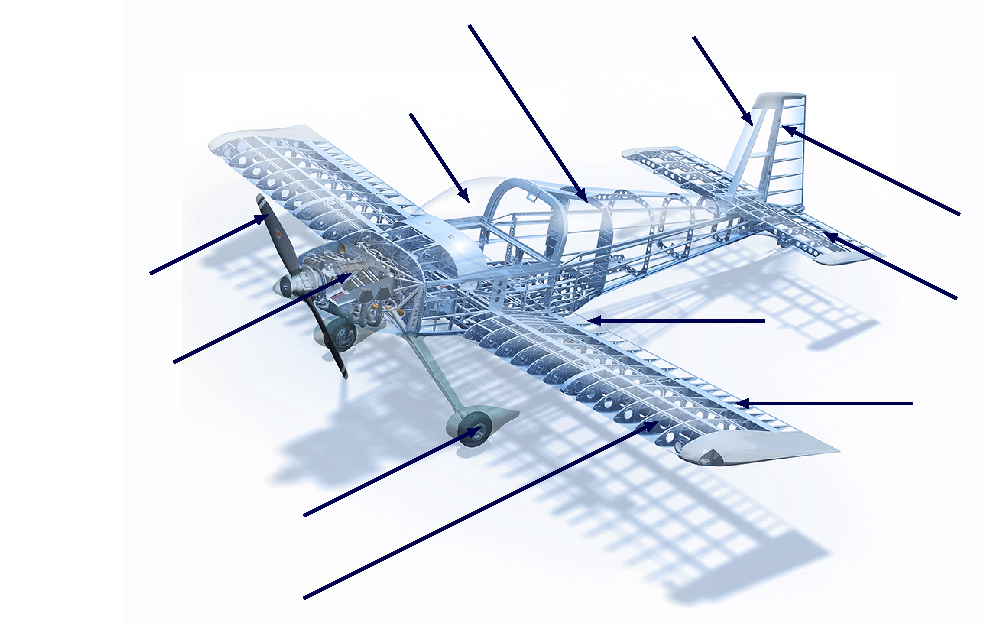
\includegraphics[scale=0.6]{01-EtudeAeronefs/img/celluleAvionNonLegendee.pdf}}
  		\only<2>{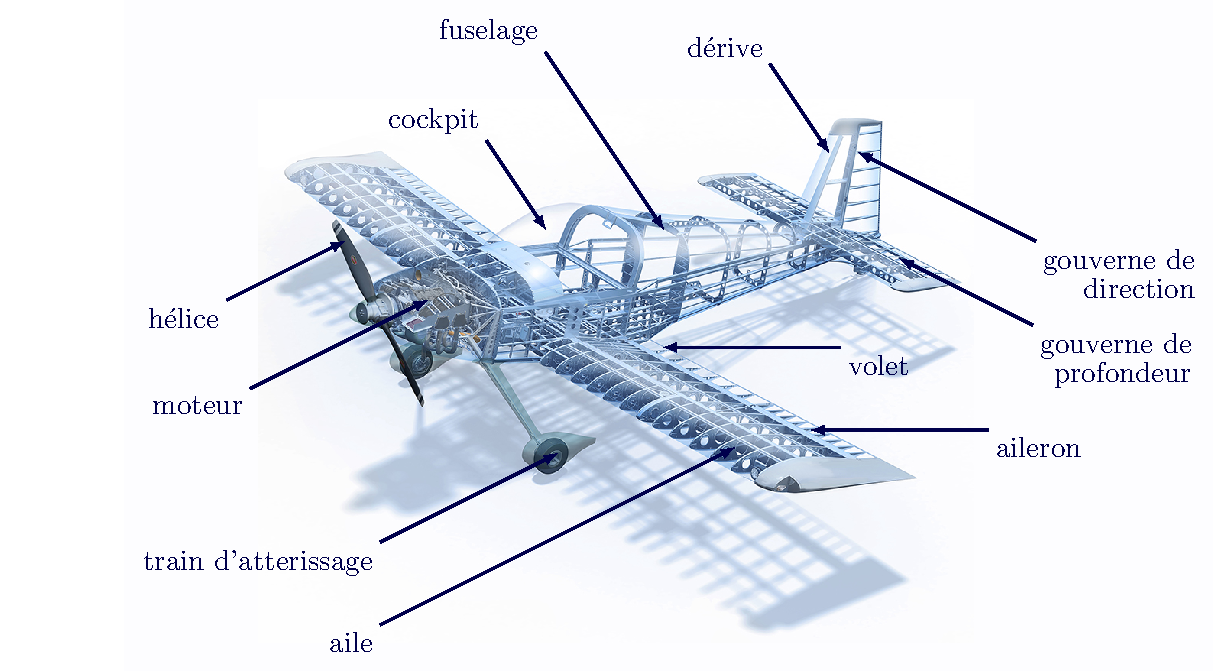
\includegraphics[scale=0.6]{01-EtudeAeronefs/img/celluleAvionLegendee.pdf}}
  		\legende{Cellule d'un avion}{img:celluleAvionLegendee}	
  		\pause
	\end{figure}
 \end{frame}
 
 \subsection{L'aile}
 \begin{frame}{Les efforts sur les structures}
 	\begin{figure}[H]
  		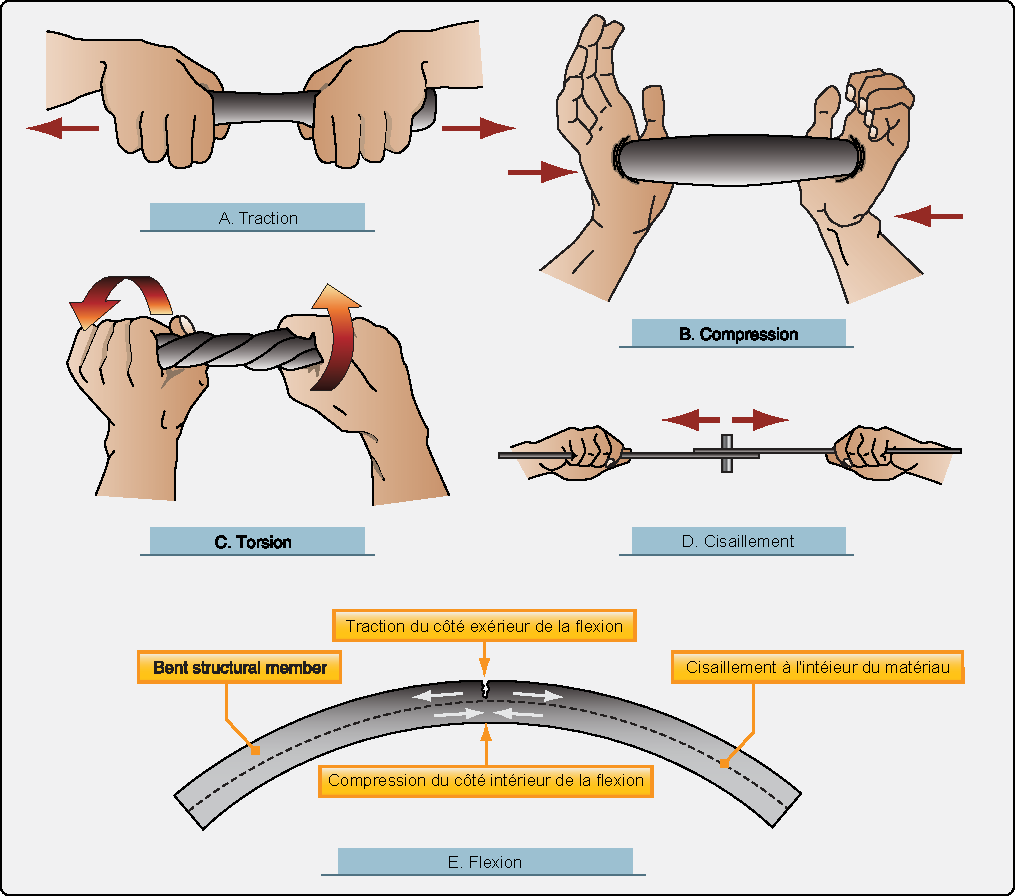
\includegraphics[width=0.55\textwidth]{01-EtudeAeronefs/img/forcesEtContraintes.pdf}
  		\legende{Les forces et contraintes}{img:forcesEtContraintes}
	\end{figure}
 \end{frame}
 
 \begin{frame}{Description générale - aile}
 	\begin{figure}[H]
  		\only<1| handout:0>{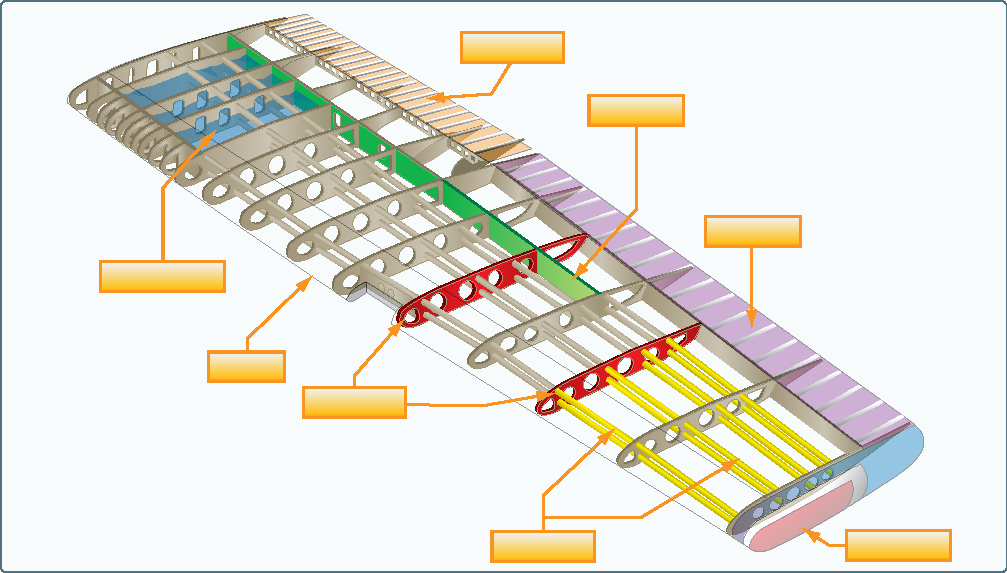
\includegraphics[scale=0.6]{01-EtudeAeronefs/img/schemaAileSansLegende.pdf}}
  		\only<2>{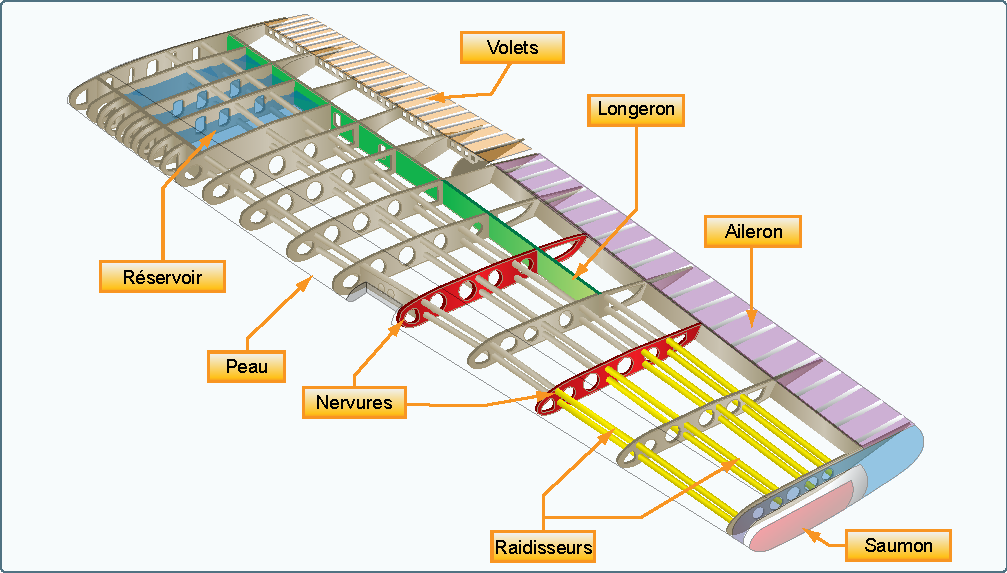
\includegraphics[scale=0.6]{01-EtudeAeronefs/img/schemaAile.pdf}}
  		\legende{Description d'une aile}{img:schemaAile}
  		\pause
	\end{figure}
 \end{frame}
 
 \begin{frame}{Matériaux d'une aile}
  \begin{columns}
  \begin{column}{0.4\textwidth}
  \begin{figure}[H]
    \only<2>{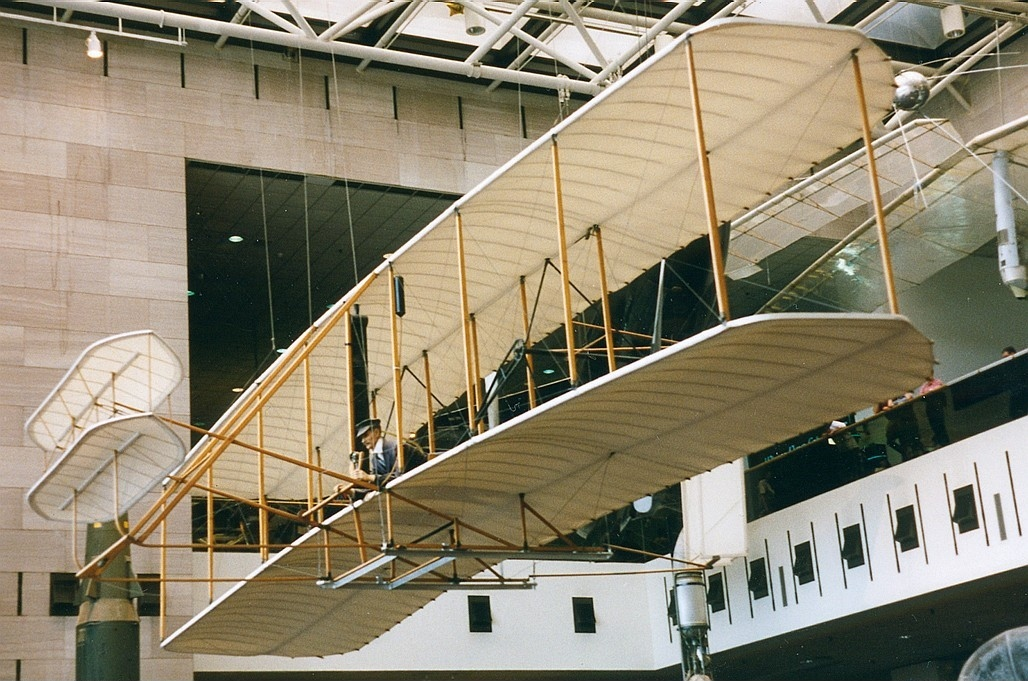
\includegraphics[width=1.15\textwidth]{05-Histoire/img/WrightFlyer_1995.jpg}
 	\legende{Wright Flyer, premier avion}{img:WrightFlyer_1995}}
 	\only<3>{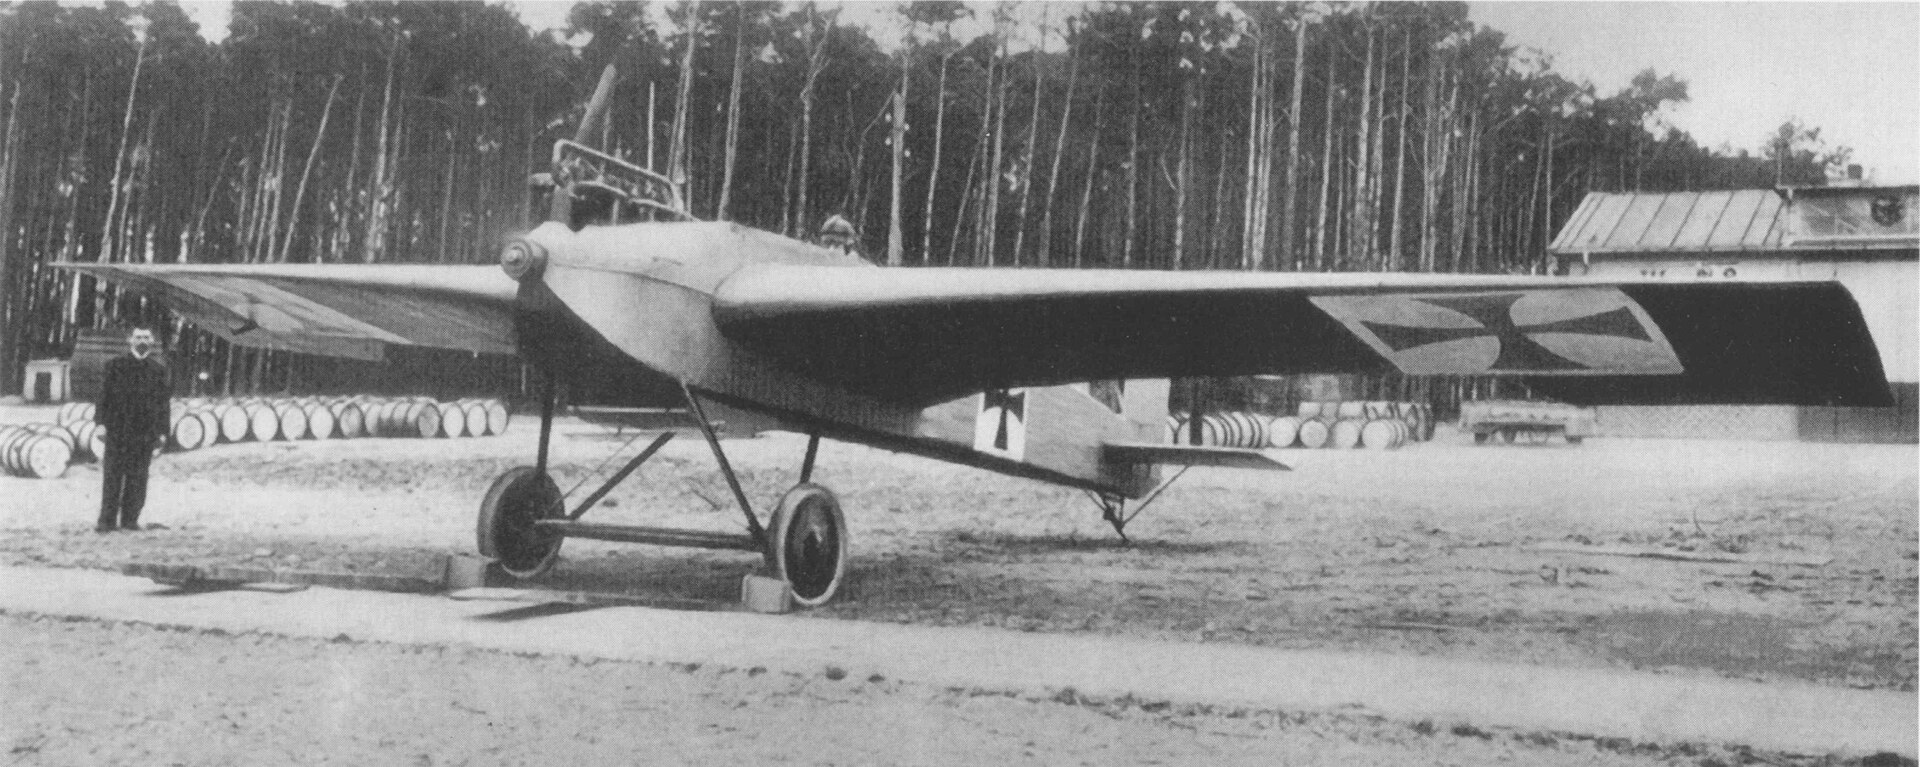
\includegraphics[width=1.15\textwidth]{01-EtudeAeronefs/img/junkerJ1.jpg}
 	\legende{Junker J1, premier avion entièrement métallique, en 1915}{img:junkerJ1}}
 	\only<4>{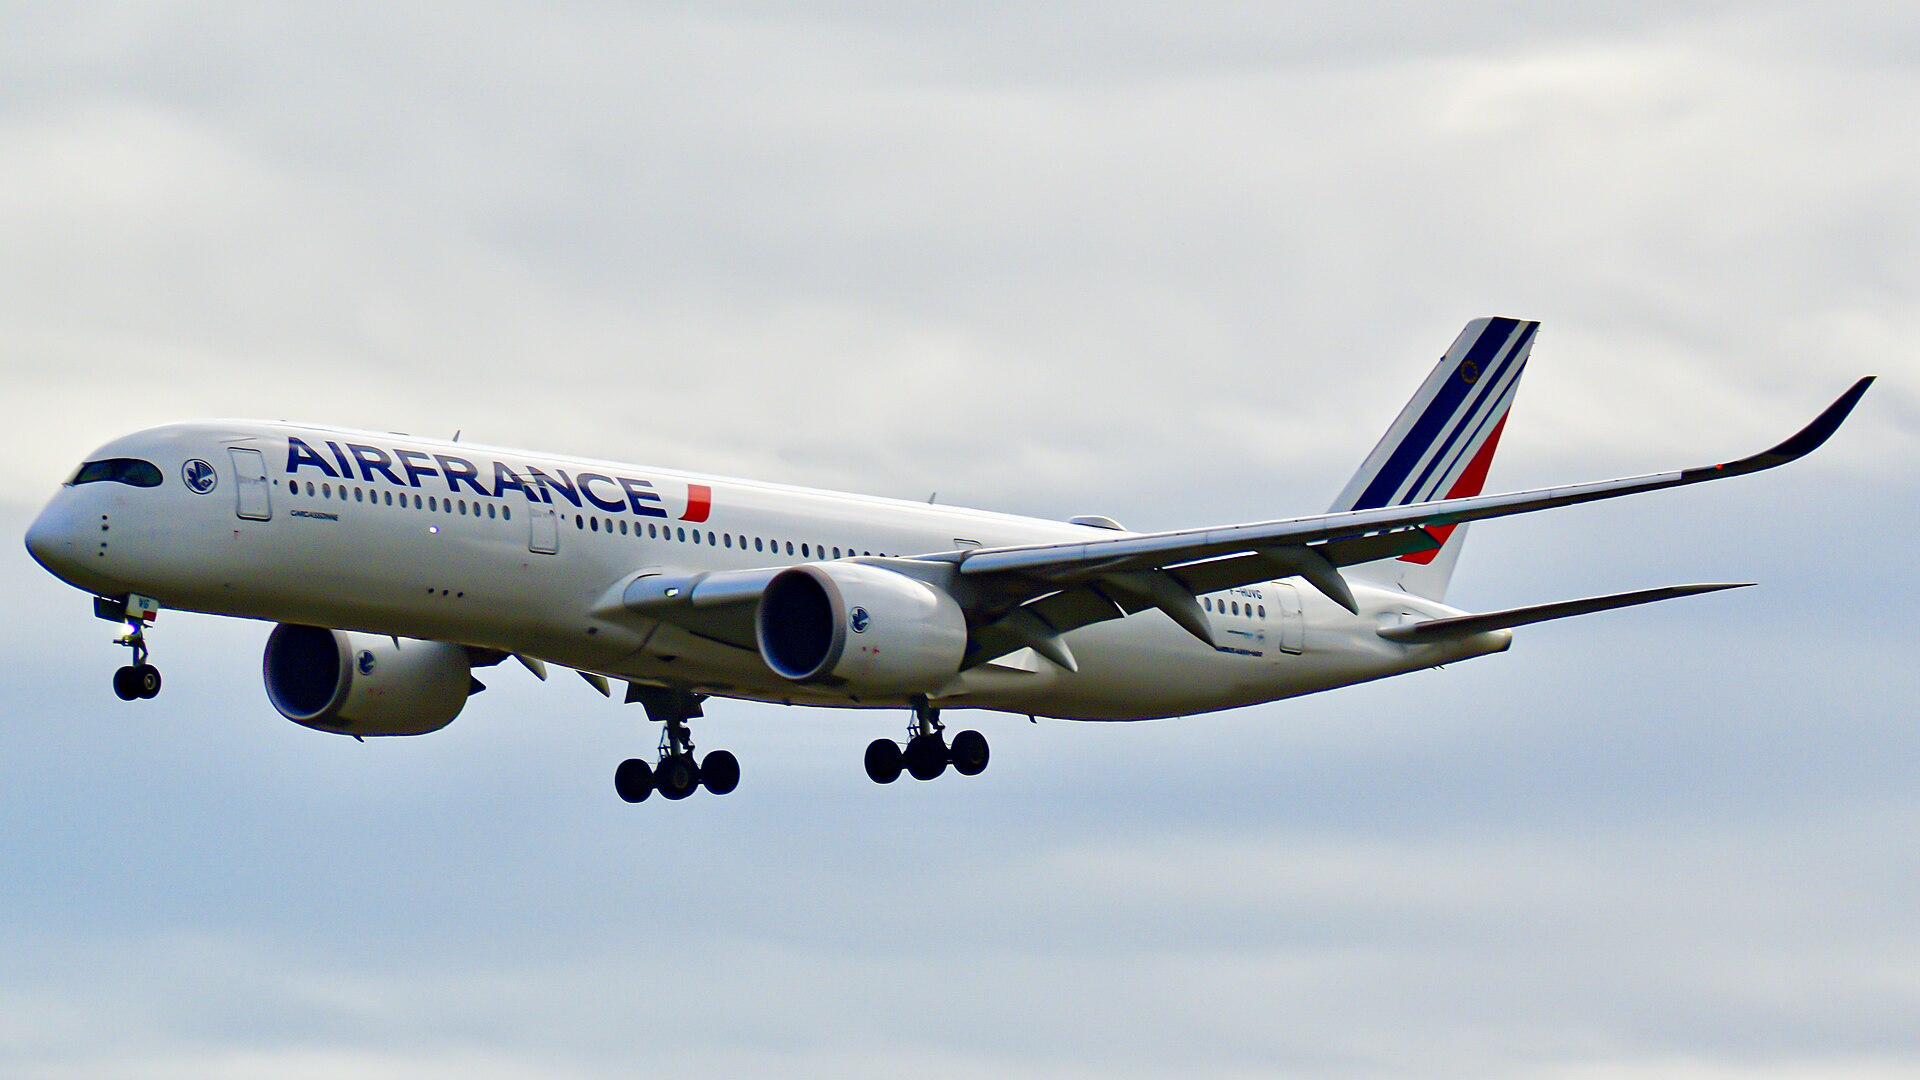
\includegraphics[width=1.15\textwidth]{01-EtudeAeronefs/img/A350.jpg}
 	\legende{Airbus A350, cellule constituée à 53\% de matériaux composites}{img:A350}}
 	\end{figure}
 \end{column}
 \begin{column}{0.6\textwidth}
 \begin{itemize}
 	\item Les premières ailes étaient des structures en \pause bois entoilées. Le bois utilisé est généralement de l'acajou, du frêne, de l'épicéa ou du sapin
 	\pause
 	\item Avec l'augmentation de la vitesse, des avions en structures métalliques sont apparues dès 1915
 	\pause
 	\item Désormais (depuis les années 1960), de plus en plus d'avions sont construits en composites : fibres de verre, polyester, et désormais carbone
 \end{itemize}
 \end{column}
 \end{columns}
 
 \end{frame}
 
 \subsection{Cellule d'un hélicoptère}
 \begin{frame}{Description générale - hélicoptère}
 	\begin{figure}[H]
  		\only<1| handout:0>{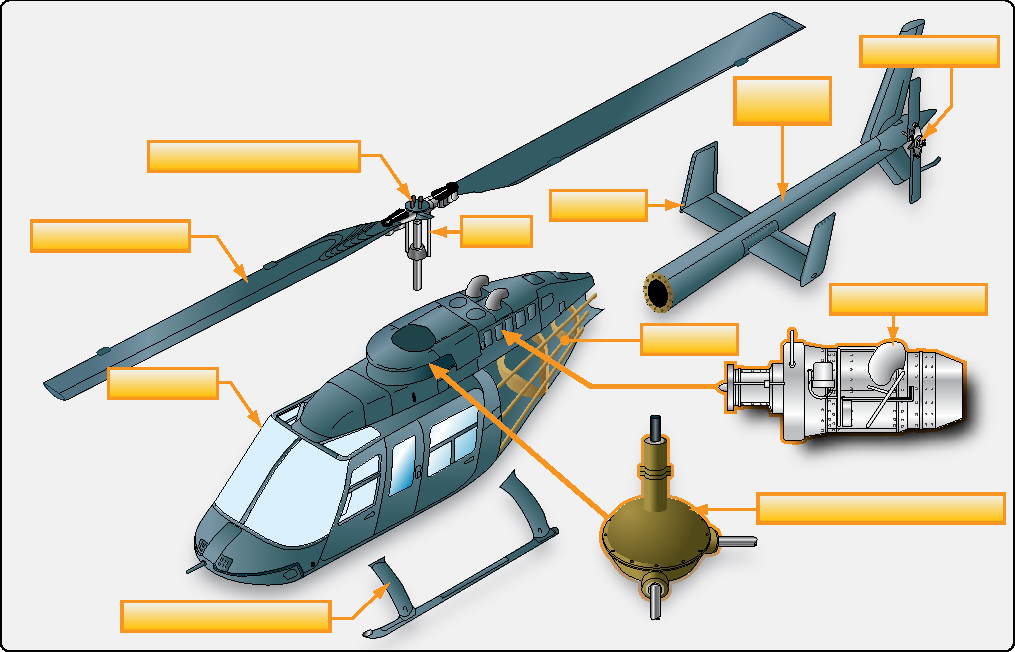
\includegraphics[width=0.76\textwidth]{01-EtudeAeronefs/img/structureHelicoptereSansLegende.pdf}}
  		\only<2>{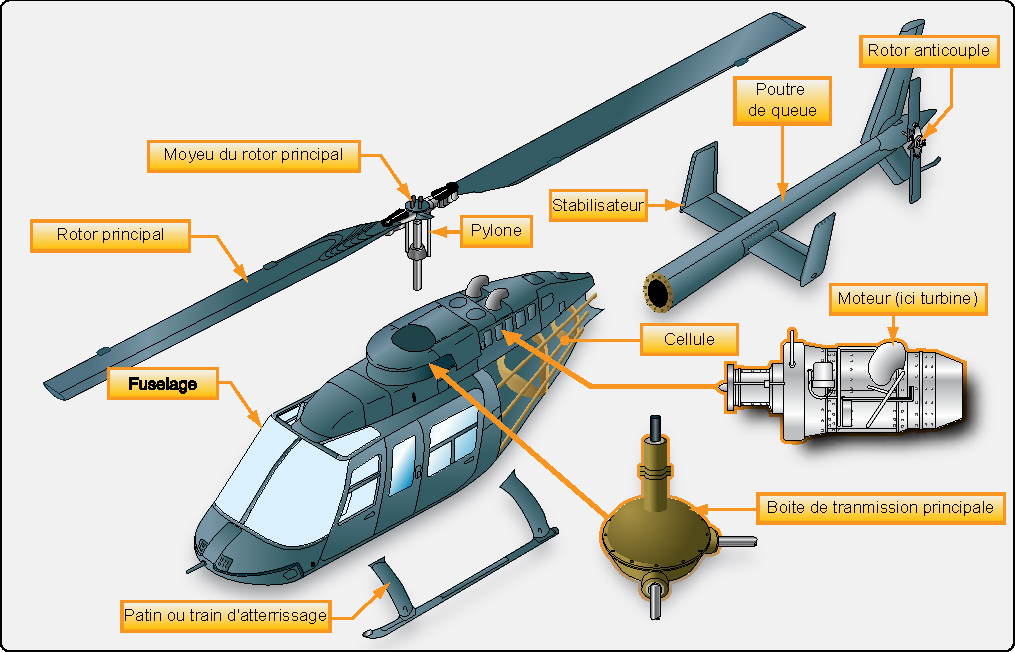
\includegraphics[width=0.76\textwidth]{01-EtudeAeronefs/img/structureHelicoptere.pdf}}
  		\legende{Composition d'un hélicoptère}{img:structureHelicoptere}
  		\pause
	\end{figure}
 \end{frame}
 
 \section{Différentes dispositions de cellules}
 \begin{frame}{Différents types de train d'atterrissage}
 
 \begin{columns}
 \begin{column}{0.5\textwidth}
 \begin{figure}[H]
  		\centering
  		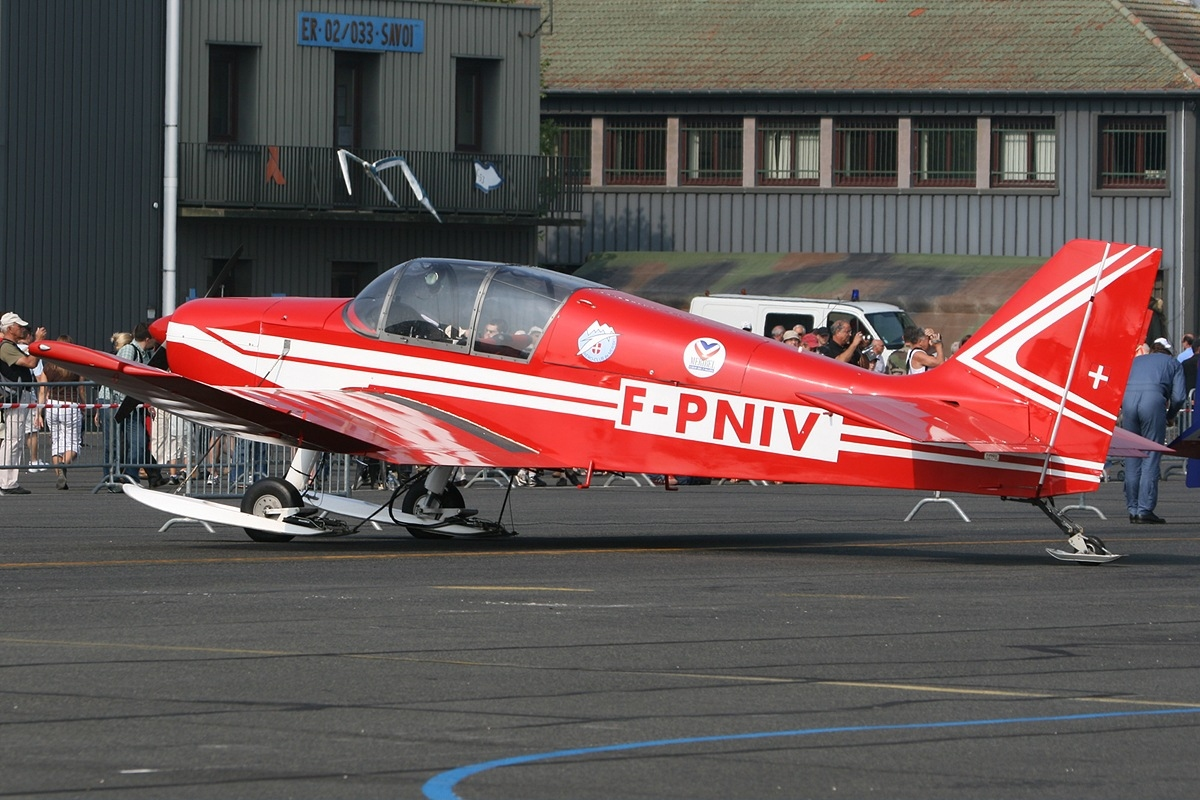
\includegraphics[width=0.95\textwidth,trim={0 2cm 0 2cm},clip]{01-EtudeAeronefs/img/D140.jpg}
  		\legende{Train classique}{img:D140}	
		\end{figure}
		\begin{itemize}
			\item disposition "historique"
			\item légèrement plus performant en vol
			\item roulage, décollage, atterrissage plus difficiles
		\end{itemize}
 \end{column}
 \begin{column}{0.5\textwidth}
 \begin{figure}[H]
  		\centering
  		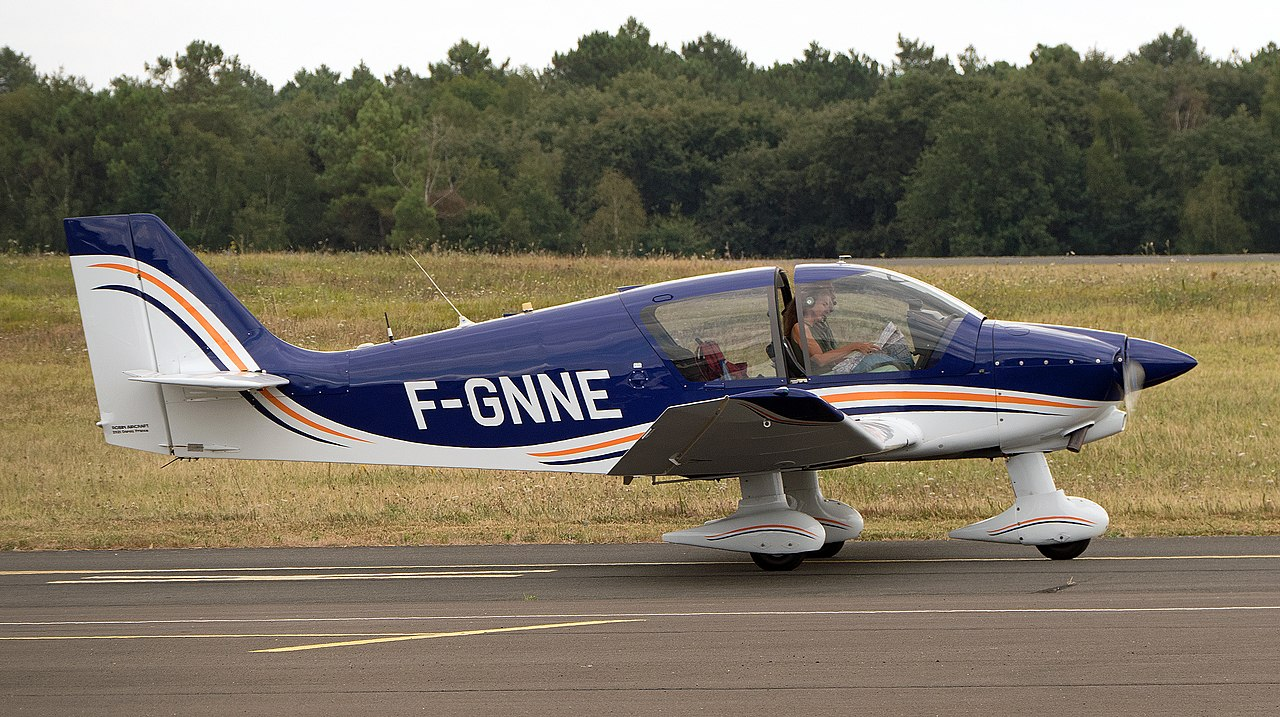
\includegraphics[width=0.95\textwidth]{01-EtudeAeronefs/img/DR400.jpg}
  		\legende{Train tricycle}{img:DR400}	
		\end{figure}
		\begin{itemize}
			\item Protège l'hélice
			\item Meilleure visibilité au sol
		\end{itemize}
 \end{column}
 \end{columns}
 
 \end{frame} 
 
 \begin{frame}{Différentes configurations d'ailes : les multiplans}
 	Au début de l'aviation, on multiplie les ailes pour augmenter la portance et la rigidité. On parle de l'ère des multiplans (par opposition aux monoplans).
 	
 \begin{columns}
 \begin{column}{0.33\textwidth}
 \begin{figure}[H]
  		\centering
  		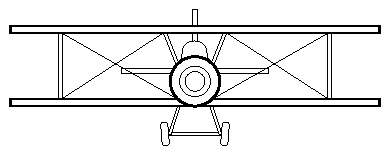
\includegraphics[width=0.95\textwidth]{01-EtudeAeronefs/img/ailes/Biplane_wire.pdf}
  		\legende{Biplan}{wing:Biplane-wire}	
		\end{figure}
 \end{column}
 \begin{column}{0.33\textwidth}
 \begin{figure}[H]
  		\centering
  		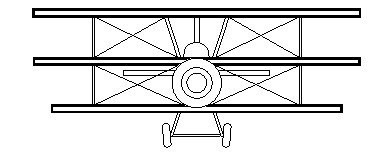
\includegraphics[width=0.95\textwidth]{01-EtudeAeronefs/img/ailes/Triplane.pdf}
  		\legende{Triplan}{wing:Triplane}	
		\end{figure}
 \end{column}
 \begin{column}{0.33\textwidth}
 \begin{figure}[H]
  		\centering
  		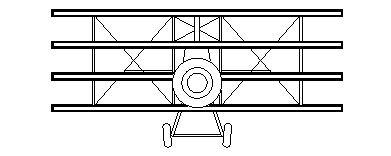
\includegraphics[width=0.95\textwidth]{01-EtudeAeronefs/img/ailes/Quadruplane.pdf}
  		\legende{Quadriplan}{wing:Quadruplane}	
		\end{figure}
 \end{column}
 \end{columns}
 
 \begin{columns}
 \begin{column}{0.33\textwidth}
 \begin{figure}[H]
  		\centering
  		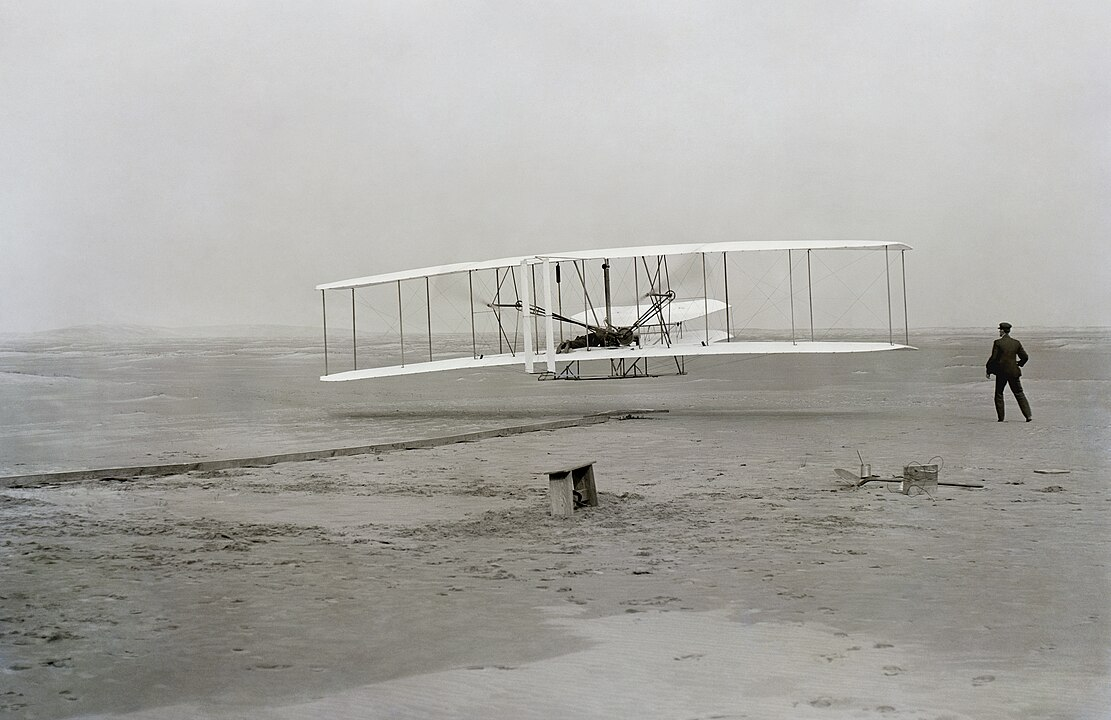
\includegraphics[width=0.8\textwidth]{05-Histoire/img/wrightFlyer.jpg}
  		\legende{Le Wright Flyer}{img:wrightFlyer}	
		\end{figure}
 \end{column}
 \begin{column}{0.33\textwidth}
 \begin{figure}[H]
  		\centering
  		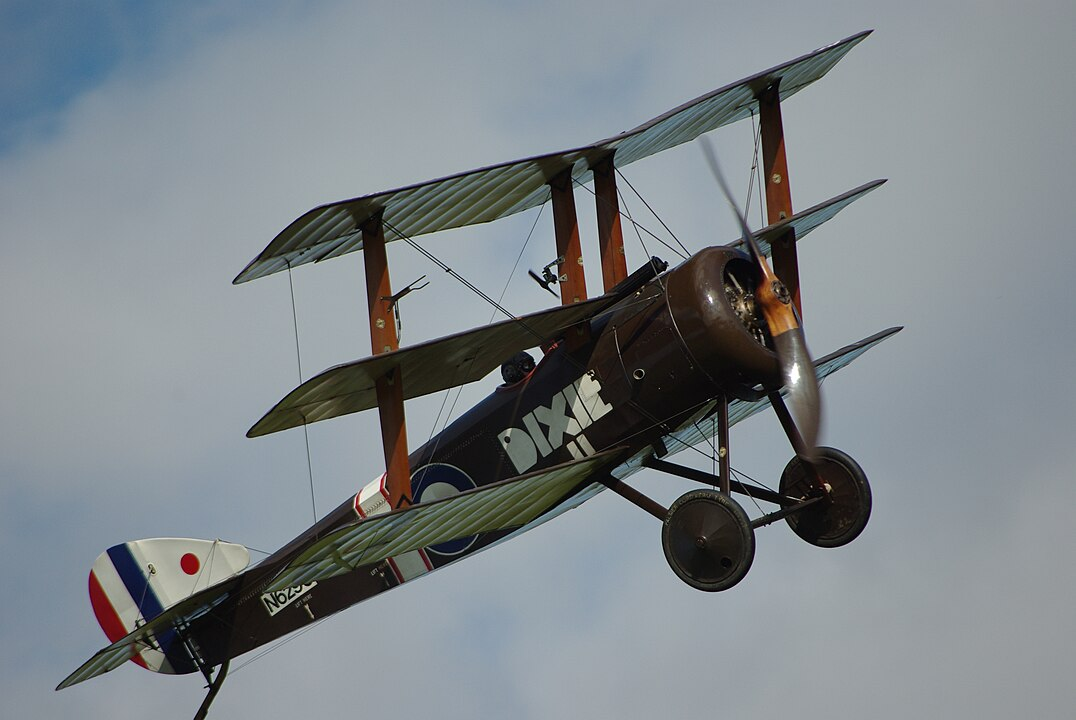
\includegraphics[width=0.8\textwidth]{05-Histoire/img/sopwithTriplane.jpg}
  		\legende{Sopwith Triplane}{img:sopwithTriplane}	
		\end{figure}
 \end{column}
 \begin{column}{0.33\textwidth}
 \begin{figure}[H]
  		\centering
  		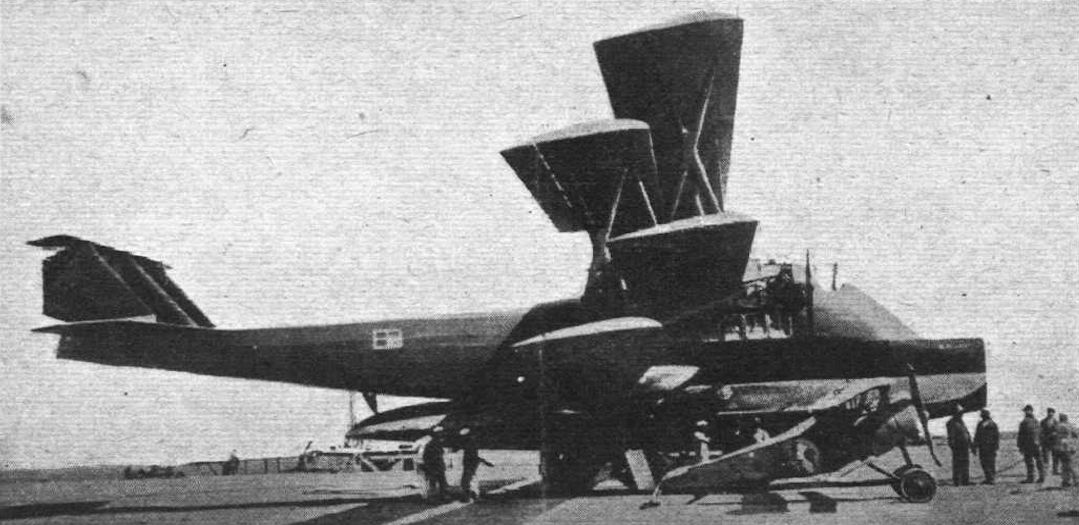
\includegraphics[width=0.95\textwidth]{05-Histoire/img/bessonH5.jpg}
  		\legende{Besson H5}{img:bessonH5}	
		\end{figure}
 \end{column}
 \end{columns}
 
 \end{frame}
 
 \begin{frame}{Différentes configurations d'ailes : le dièdre}
	Le dièdre est l'angle formé par le plan de chaque aile et le plan horizontal. Il peut être positif, nul ou négatif. Le dièdre a un impact sur la stabilité.
 
 \begin{columns}
 \begin{column}{0.33\textwidth}
 \begin{figure}[H]
  		\centering
  		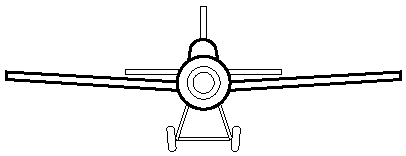
\includegraphics[width=0.95\textwidth]{01-EtudeAeronefs/img/ailes/Monoplane_dihedral.pdf}
  		\legende{Dièdre positif}{wing:Monoplane-dihedral}	
		\end{figure}
 \end{column}
 \begin{column}{0.33\textwidth}
 \begin{figure}[H]
  		\centering
  		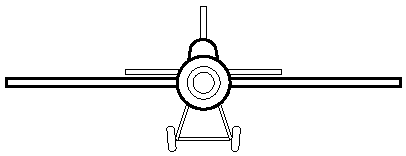
\includegraphics[width=0.95\textwidth]{01-EtudeAeronefs/img/ailes/Monoplane_mid.pdf}
  		\legende{Dièdre nul}{wing:Monoplane-mid}	
		\end{figure}
 \end{column}
 \begin{column}{0.33\textwidth}
 \begin{figure}[H]
  		\centering
  		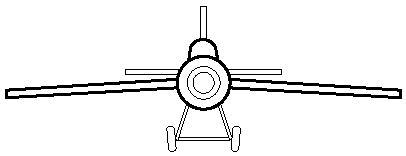
\includegraphics[width=0.95\textwidth]{01-EtudeAeronefs/img/ailes/Monoplane_anhedral.pdf}
  		\legende{Dièdre négatif}{wing:Monoplane-anhedral}	
		\end{figure}
 \end{column}
 \end{columns}
 
 \end{frame}
 
 \begin{frame}{Différentes configurations d'ailes : différentes configurations}
	Il existe de nombreuses formes d'ailes. En voici quelques-unes.
 
 \begin{columns}
 \begin{column}{0.33\textwidth}
 \begin{figure}[H]
  		\centering
  		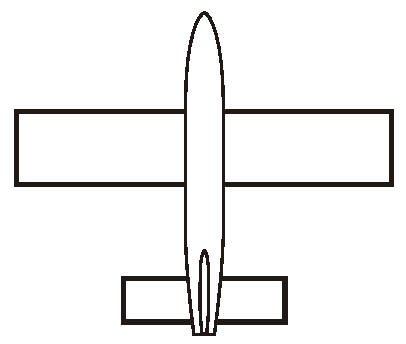
\includegraphics[width=0.95\textwidth]{01-EtudeAeronefs/img/ailes/Wing_constant.pdf}
  		\legende{Aile rectangulaire}{wing:Wing-constant}	
		\end{figure}
 \end{column}
 \begin{column}{0.33\textwidth}
 \begin{figure}[H]
  		\centering
  		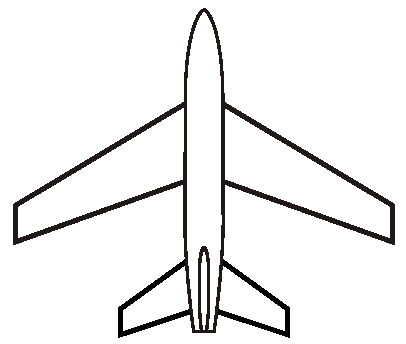
\includegraphics[width=0.95\textwidth]{01-EtudeAeronefs/img/ailes/Wing_swept.pdf}
  		\legende{Aile en flèche}{wing:Wing-swept}	
		\end{figure}
 \end{column}
 \begin{column}{0.33\textwidth}
 \begin{figure}[H]
  		\centering
  		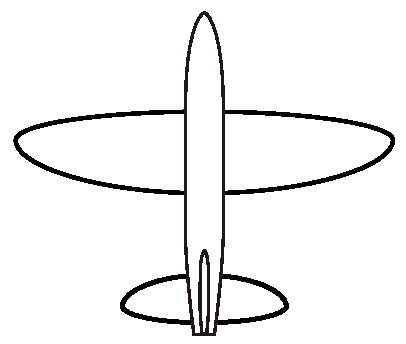
\includegraphics[width=0.95\textwidth]{01-EtudeAeronefs/img/ailes/Wing_elliptical.pdf}
  		\legende{Aile elliptique}{wing:Wing-elliptical}	
		\end{figure}
 \end{column}
 \end{columns}
 \end{frame}
 
 \begin{frame}{Différentes configurations d'ailes : différentes configurations}
	Il existe de nombreuses formes d'ailes. En voici quelques-unes.
 
 \begin{columns}
 \begin{column}{0.33\textwidth}
 \begin{figure}[H]
  		\centering
  		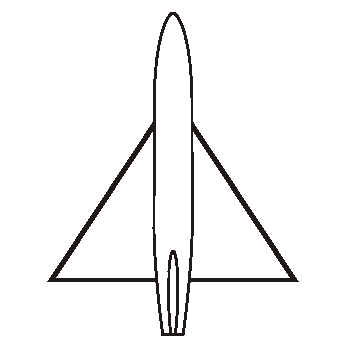
\includegraphics[width=0.95\textwidth]{01-EtudeAeronefs/img/ailes/Wing_tailless_delta.pdf}
  		\legende{Aile delta}{wing:Wing-tailless-delta}	
		\end{figure}
 \end{column}
 \begin{column}{0.33\textwidth}
 \begin{figure}[H]
  		\centering
  		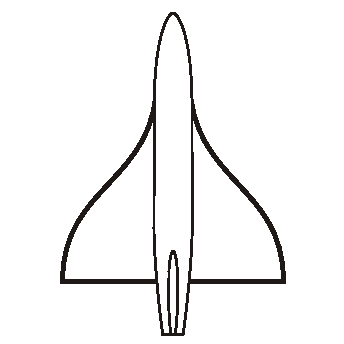
\includegraphics[width=0.95\textwidth]{01-EtudeAeronefs/img/ailes/Wing_ogival_delta.pdf}
  		\legende{Aile gothique}{wing:Wing-ogival-delta}	
		\end{figure}
 \end{column}
 \begin{column}{0.33\textwidth}
 \begin{figure}[H]
  		\centering
  		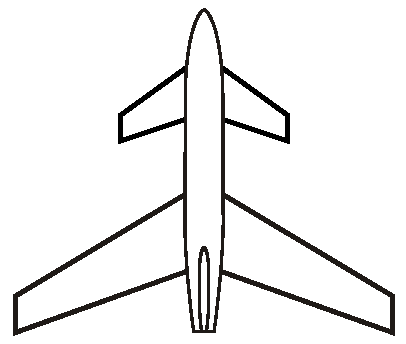
\includegraphics[width=0.95\textwidth]{01-EtudeAeronefs/img/ailes/Wing_canard.pdf}
  		\legende{Configuration canard}{wing:Wing-canard}	
		\end{figure}
 \end{column}
 \end{columns}
 \end{frame}
 
 \begin{frame}{Différentes configurations d'ailes : différentes configurations}
	Il existe de nombreuses formes d'ailes. En voici quelques-unes.
 
 \begin{columns}
 \begin{column}{0.33\textwidth}
 \begin{figure}[H]
  		\centering
  		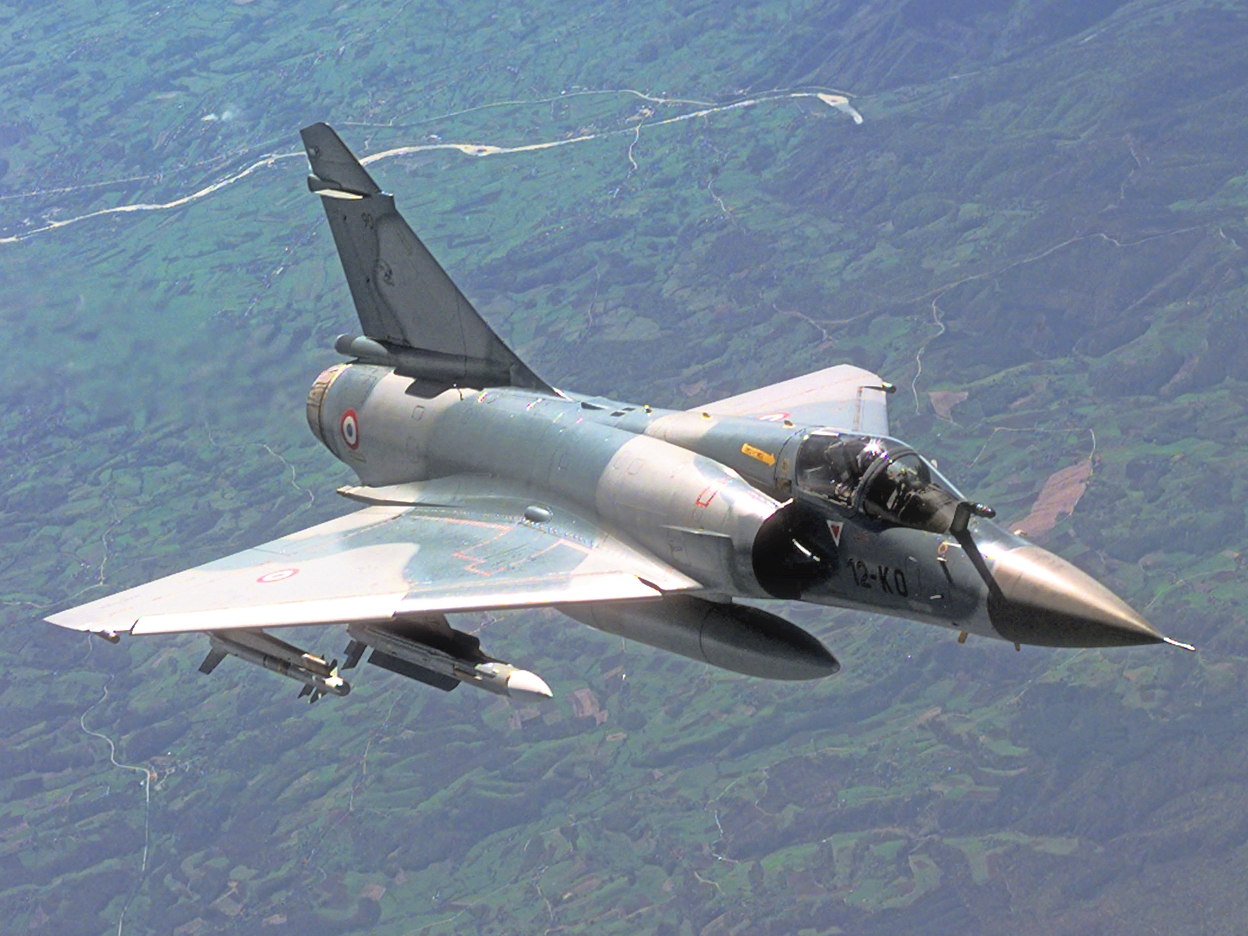
\includegraphics[width=0.95\textwidth]{01-EtudeAeronefs/img/mirage2000.jpg}
  		\legende{Aile delta : chasseur}{img:mirage2000}	
		\end{figure}
 \end{column}
 \begin{column}{0.33\textwidth}
 \begin{figure}[H]
  		\centering
  		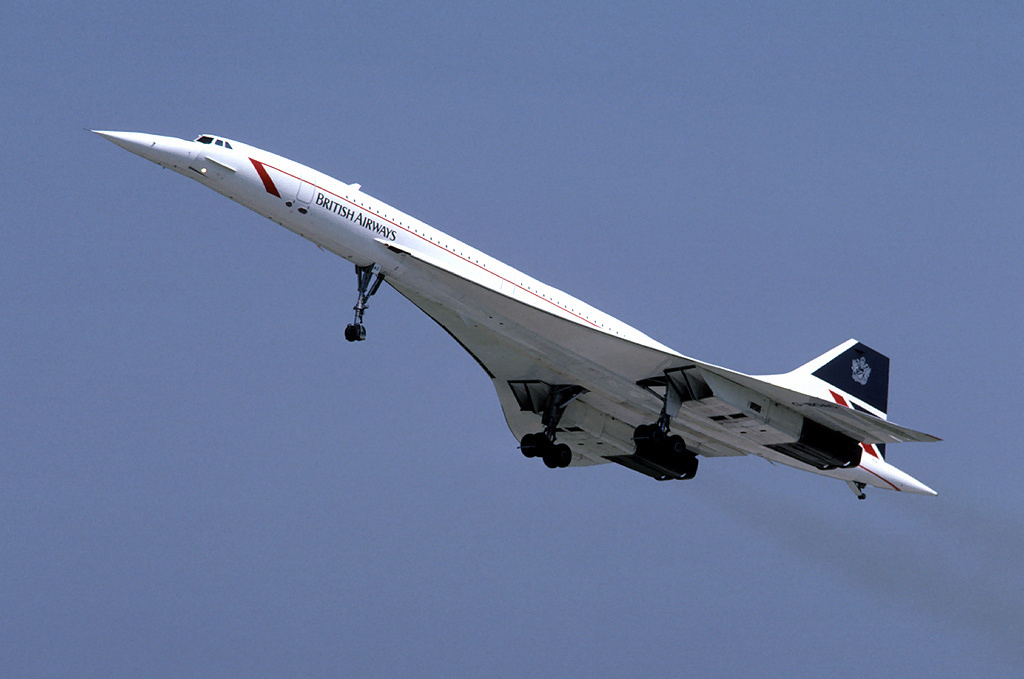
\includegraphics[width=0.95\textwidth]{01-EtudeAeronefs/img/concorde.jpg}
  		\legende{Aile gothique : Concorde}{img:concorde}	
		\end{figure}
 \end{column}
 \begin{column}{0.33\textwidth}
 \begin{figure}[H]
  		\centering
  		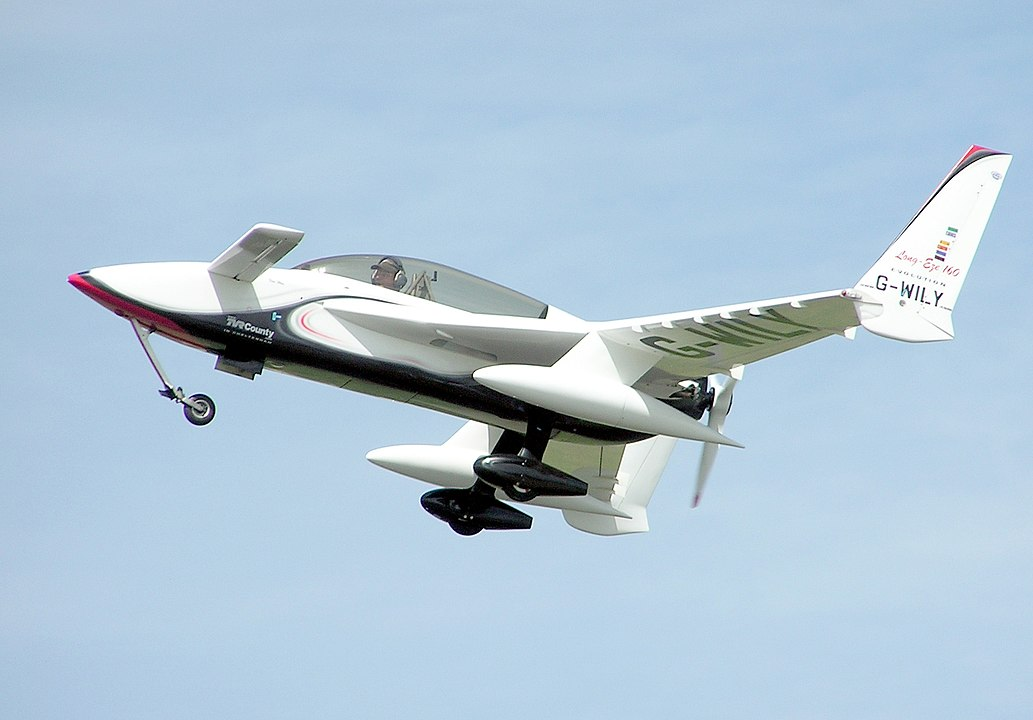
\includegraphics[width=0.95\textwidth]{01-EtudeAeronefs/img/rutanLongEz.jpg}
  		\legende{Canard : Long EZ}{img:rutanLongEz}	
		\end{figure}
 \end{column}
 \end{columns}
 \end{frame}
 
 
 
\appendix 
\section{QCM}
 \qmcBia{Étude des aéronefs}
{3}{Dans un moteur à 4 temps, la compression intervient après :}
{la combustion}
{la détente}
{l'admission}
{l'échappement}
{}

 \qmcBia{Étude des aéronefs}
{2}{Durant un cycle de fonctionnement d'un moteur à pistons (4 temps), le seul temps où le piston monte du point mort bas au point mort haut avec les soupapes fermées est le temps :}
{d'admission}
{de compression}
{de combustion-détente}
{d'échappement}
{}

\qmcBia{Étude des aéronefs}
{3}{Sur un avion certifié, un moteur à pistons contenant 4 cylindres est pourvu au total de :}
{2 bougies d'allumage}
{4 bougies d'allumage}
{8 bougies d'allumage}
{0 bougie d'allumage}
{}

\qmcBia{Étude des aéronefs}
{3}{\begin{figure}[H]
  		\centering
    		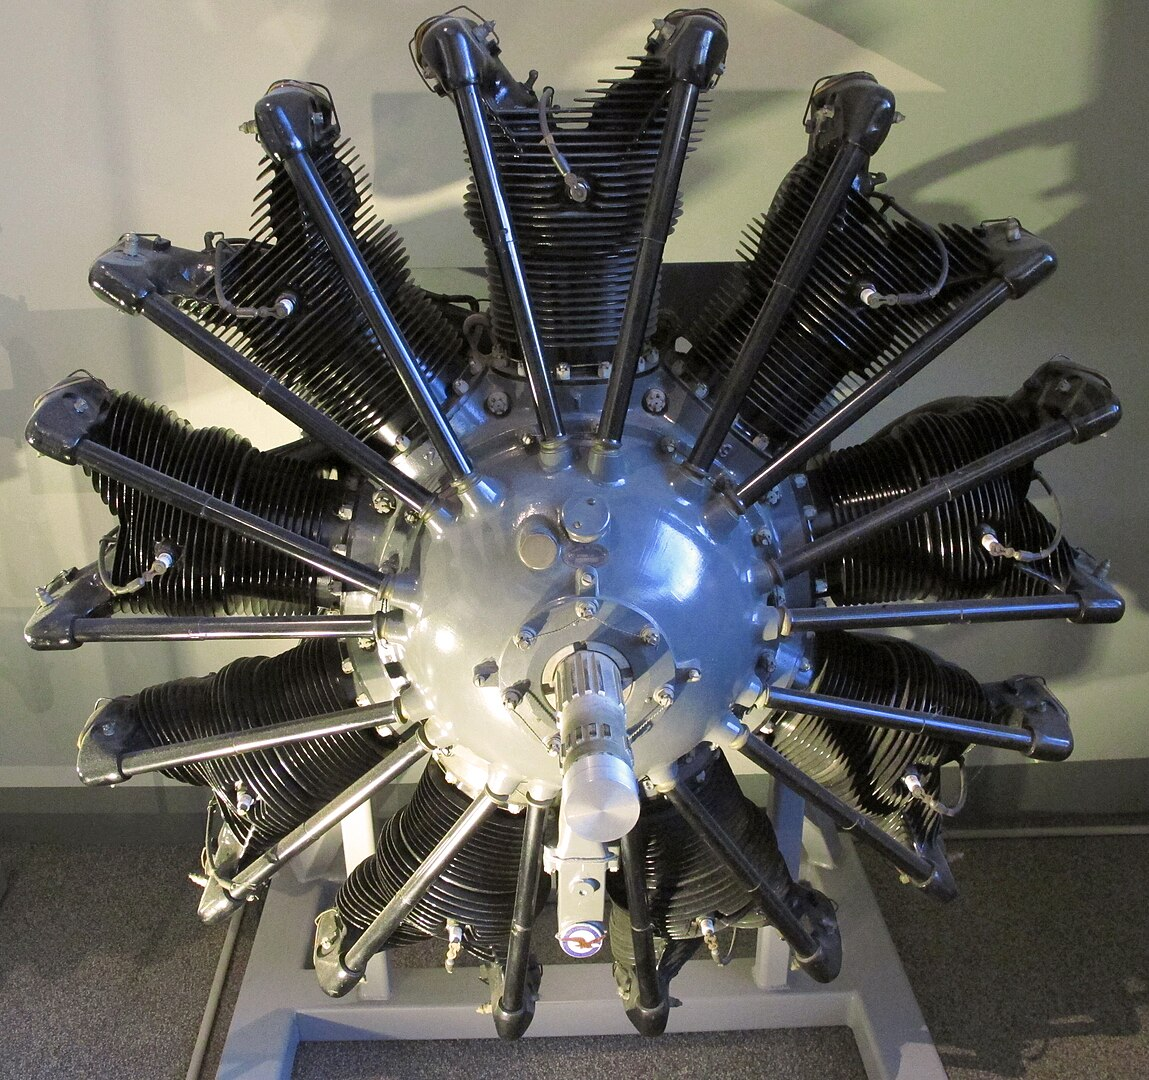
\includegraphics[width=0.2\textwidth]{01-EtudeAeronefs/img/PWWasp.jpg}
	\end{figure}	
	La disposition des cylindres de ce moteur est :}
{en ligne}
{en V}
{en étoile}
{à plat} 
{}

\qmcBia{Étude des aéronefs}
{4}{Un turbopropulseur}
{est un pulsoréacteur précédé d'un réducteur et d'une hélice}
{est un statoréacteur précédé d'un réducteur et d'une hélice}
{est un moteur à pistons équipé d'un turbocompresseur}
{est un turboréacteur précédé d'un réducteur et d'une hélice} 
{}


\qmcBia{Étude des aéronefs}
{3}{\begin{figure}[H]
  		\centering
    		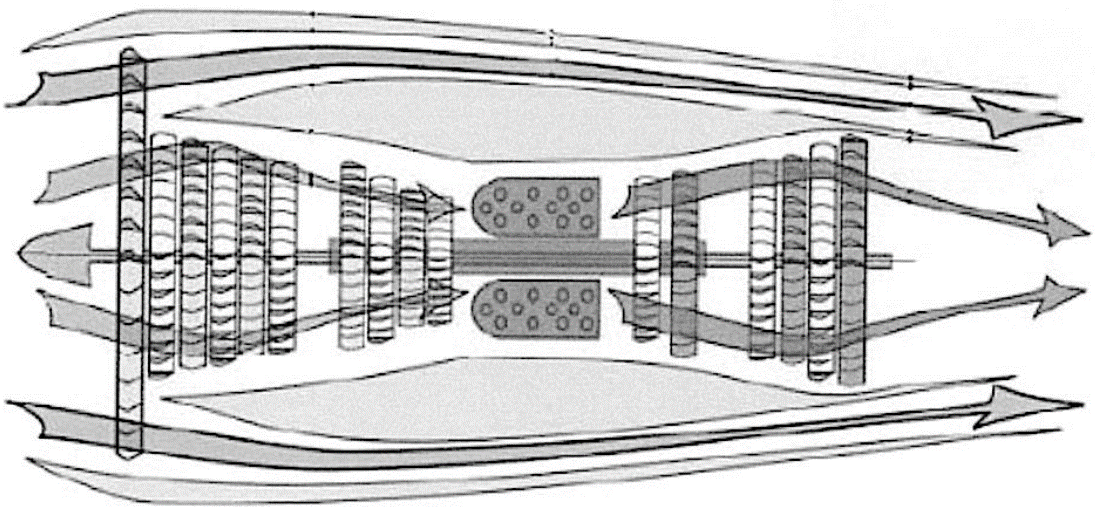
\includegraphics[width=0.4\textwidth]{imgPresentations/bia2024Q3.20.png}
	\end{figure}	
	Quel est le type de moteur de la photo ci-dessus ?}
{Turboréacteur double corps et simple flux}
{Turboréacteur simple corps et double flux}
{Turboréacteur double corps et double flux}
{Turboréacteur simple corps et simple flux} 

\qmcBia{Étude des aéronefs}
{2}{La présence d'un réchauffage de carburateur est nécessaire pour :}
{Améliorer son fonctionnement à froid}
{Pallier la formation de glace dans le venturi}
{Échauffer le mélange avant d'entrer dans les cylindres, et donc, améliorer sa combustion}
{Démarrer le moteur} 

 
\ifdefined\activerbibliobeamer
\begin{frame}[allowframebreaks]
\frametitle{Bibliographie}
\printbibliography
%\nocite{*}
\end{frame}
\fi 
 
\end{document}
